\chapter{Exemple de rapport généré par GreenT}\label{apendixReport}
\begin{figure}[H]
\centering
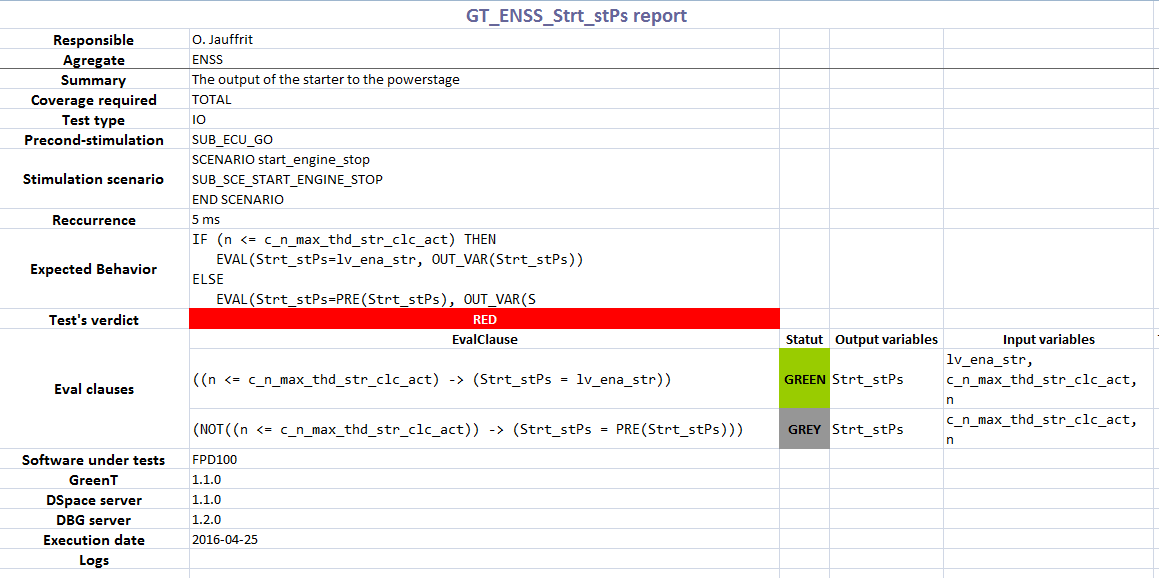
\includegraphics[width=16cm]{contents/images/report0.png}

\caption{Exemple d'un extrait de rapport généré par \textit{GreenT} -- Onglet \textit{Summary}}
\end{figure}
\begin{figure}[H]
\centering
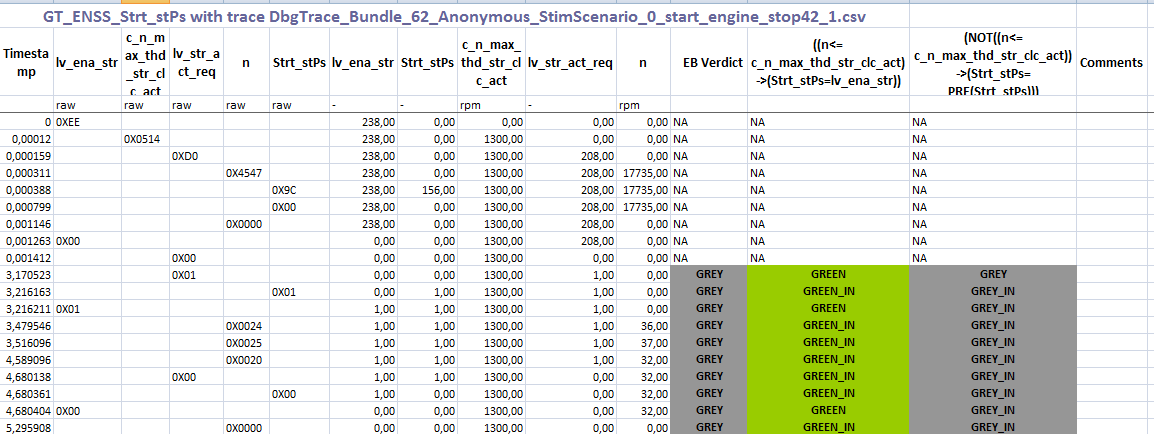
\includegraphics[width=16cm]{contents/images/report.png}
\caption{Exemple d'un extrait de rapport généré par \textit{GreenT} -- Onglet \textit{trace}}
\end{figure}
Ce rapport est un rapport vérifiant que la variable \texttt{EnvT\_tSens=temp\_air\_mes[2]}, moyennant une tolérance. 

\begin{itemize}
\item Dans la colonne A, nous avons le timestamp, le temps durant lequel la valeur a été enregistrée
\item Dans les colonnes B et C, nous avons la valeur de nos variables, en physique, c'est-à-dire converties par \textit{GreenT}
\item Dans les colonnes D et E, c'est la valeur hexadécimal, c'est-à-dire la valeur enregistrée. Cette valeur est reportée dans le rapport uniquement au moment ou elle à changé. ça peut permettre à l'utilisateur de connaître les instants ou une variable est modifiée.
\item Et enfin, dans la colonne F, le résultat de l'évaluation pour chaque instant de la trace; En l'occurence, il est toujours \textit{GREEN}.
\end{itemize}